\chapter{Inleiding}\label{ch:introductie}

Eiwitten of proteïnen zijn alomtegenwoordig en spelen een essentiële rol in ons dagelijkse leven.
Ze garanderen de correcte werking van processen binnen ons eigen lichaam, maar ook in dieren, planten, bacteriën en zelfs virussen.
Om deze processen te analyseren zijn er meerdere benaderingen mogelijk.


\section{Genomica, transcriptomica \& proteomica}\label{sec:genomica-transcriptomica-&-proteomica}
De eerste mogelijke discipline is \textbf{genomica}, het onderzoek naar het genoom.
Het genoom bestaat uit al het DNA dat aanwezig is in een organisme.
Het DNA bevat het ``recept'' voor alle proteïnen die mogelijks door het organisme geconstrueerd kunnen worden.
Dit is het begin van het centraal dogma van de biologie.
Dit centraal dogma beschrijft de omzetting van DNA naar proteïnen.
Wanneer we gebruikmaken van een analogie, dan is het DNA een receptenboek en is een proteïne een afgewerkt gerecht (waarvoor de instructies in het receptenboek staan).
Het DNA stelt dus de instructies voor van alle mogelijke proteïnen die een bepaald organisme kan maken.
Het geeft dus geen informatie over de proteïnen die op dat moment in de tijd actief zijn.
Het is een voorstelling van wat het organisme kan, niet wat het op \textit{dit} moment aan het doen is.
Belangrijk is dat ongeveer 98\% van het menselijke genoom niet-coderend is.
Dit wil zeggen dat het grootste deel van het DNA niet omgezet kan worden naar een betekenisvolle proteïne.
In de plaats kunnen deze niet-coderende delen omgezet worden naar \textit{regulatory sequences}, niet-coderende genen, of andere componenten waarvan we nog niet altijd weten of ze al dan niet een functie hebben.
\\ \\
De tweede discipline is de \textbf{transcriptomica}.
Deze discipline onderzoekt het transcriptoom van een organisme.
Dit is de verzameling van alle RNA moleculen die in het organisme aanwezig zijn.
Het transcriptoom is een belangrijke indicator voor welke delen uit het DNA effectief proteïnen encoderen.
Dit komt omdat RNA, meer specifiek messenger RNA (mRNA) en transfer RNA (tRNA), een belangrijk onderdeel zijn van het proces om DNA om te zetten naar proteïnen.
In de restaurant analogie is dit een kopie van één recept uit het receptenboek.
Dit recept beschrijft hoe het gerecht exact gemaakt moet worden.
\\ \\
Tot slot bestaat ook het onderzoeksgebied van de \textbf{proteomica}.
Dit is de studie van alle proteïnen die binnen een enkel organisme tot expressie kunnen komen.
Hierbij probeert men te begrijpen hoe proteïnen in elkaar zitten, hoe deze binnen een bepaalde omgeving met elkaar interageren en wat hun belangrijkste functie is.
Het voordeel van het bestuderen van de proteïnen is dat je weet welke proteïnen exact op een specifiek moment aanwezig zijn.
Op die manier kan men afleiden wat er exact gebeurt in een organisme.
Zoals eerder beschreven zijn de proteïnen het afgewerkte gerecht binnen onze analogie.
Een visualisatie van het centraal dogma van de biologie, inclusief de link met de gebruikte analogie, kan teruggevonden worden in Figuur~\ref{fig:recipe}~\cite{image_central_dogma}.
\\ \\
De focus van deze masterproef ligt vooral binnen het veld van de \textbf{metaproteomica}.
Het prefix \textit{meta} geeft aan dat de te analyseren stalen niet van één organisme afkomstig zijn, maar van \textbf{meerdere organismen} (typisch binnen hetzelfde ecosysteem).
Dit maakt de analyse moeilijker aangezien proteïnen van verschillende organismen gelijkaardige aminozuursequenties kunnen hebben (al dan niet door toeval).
Binnen het metaproteomica veld gaan onderzoekers op zoek naar welke organismes er in een ecosysteem aanwezig zijn en wat deze daar dan doen.
Dit doet men door een verzameling van proteïnefragmenten te analyseren.
Deze proteïnefragmenten noemen we peptiden wanneer ze bestaan uit twee of meer aminozuren en hun lengte beperkt blijft.
In de praktijk gaat dit over sequenties van ongeveer 2 tot 50 aminozuren lang.
Idealiter kunnen we deze analyses uitvoeren met volledige proteïnen, en niet met peptiden.
Dit is echter niet mogelijk vanwege beperkingen bij de huidige generatie aan machines die proteïnen inlezen.
Deze kunnen slechts korte fragmenten (peptiden) inlezen.
Een veelvoorkomende categorie van peptiden die we zullen analyseren zijn tryptische peptiden.

\begin{figure}[H]
    \centering
    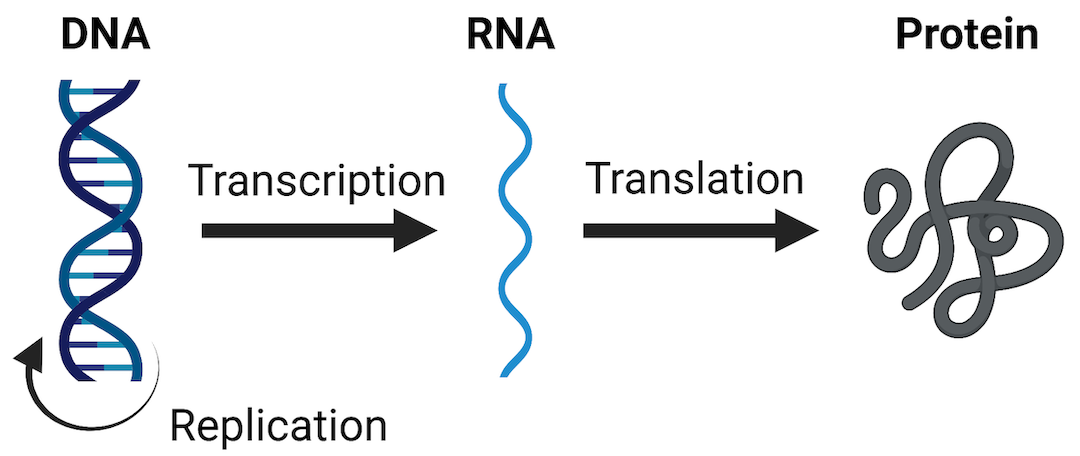
\includegraphics[width=0.6\textwidth]{central_dogma}
    \caption{Visualisatie van het centraal dogma van de biologie~\cite{image_central_dogma}. Gebruikmakende van een analogie kunnen we het DNA vergelijken met een receptenboek. Eén kopie van één recept komt overeen met RNA. Een afgewerkt gerecht komt dan weer overeen met een proteïne.}
    \label{fig:recipe}
\end{figure}


\section{Tryptische peptiden}\label{sec:tryptische-peptiden}
Tryptische peptiden ontstaan na het knippen van proteïnen aan de hand van \textbf{trypsine}.
Dit is een protease (eiwitafbrekend enzym) dat proteïnen opsplitst in meerdere peptiden.
Er bestaan nog andere proteases, maar trypsine is veruit de populairste door zijn eenduidig gedrag en efficiëntie.
\\ \\
Trypsine zal proteïnen knippen na elk voorkomen van lysine (K) of arginine (R) indien het eerstvolgende aminozuur geen proline (P) is.
Deze vuistregel is echter niet perfect.
Soms mist trypsine een locatie waar volgens deze regel geknipt moet worden.
Dit noemen we een \textit{missed cleavage}.
Figuur~\ref{fig:trypsine} bevat een voorbeeld van de werking.

\begin{figure}[H]
    \centering
    \includesvg[width=0.9\textwidth]{trypsine_verwerking}
    \caption{Voorbeeld van de werking van trypsine op 2 proteïnen~\cite{phdPieterUnipept}. De aminozuren in het rood zijn lysine (K) of arginine (R), waarna trypsine knipt (behalve als het eerstvolgende aminzoruur proline (P) is). De tweede proteïne bevat een voorbeeld waar niet geknipt wordt na lysine, doordat het volgende aminozuur proline is.}
    \label{fig:trypsine}
\end{figure}

Om de peptiden uit een experiment te kunnen gebruiken bij computeranalyses moeten deze omgezet worden naar een stringrepresentatie.
Dit is is echter een moeilijk en ingewikkeld proces.
Eerst wordt de massa/ladingsverhouding (m/z) van peptiden aan de hand van een massaspectrometer gemeten.
Daarna worden deze resultaten aan de hand van diverse zoekprocessen (via zogenaamde zoekmachines) omgezet naar de stringvoorstelling van de peptide.
Deze sequenties vormen de input voor tools zoals Unipept.
\\ \\
Eén belangrijke consequentie van het gebruik van een massaspectrometer is dat isoleucine (I) en leucine (L) niet uit elkaar gehouden kunnen worden.
Deze aminozuren bestaan uit dezelfde atomen (C\textsubscript{6}H\textsubscript{13}NO\textsubscript{2}), maar hebben niet dezelfde structuur.
Bijgevolg hebben ze een identieke massa, en zijn ze niet te onderscheiden van elkaar.


\section{Unipept}\label{sec:unipept-introductie}
Unipept~\cite{unipept_orig} biedt een ecosysteem van tools aan om stalen uit het onderzoeksveld van de metaproteomica te analyseren, maar er is ook een onderdeel (UMGAP~\cite{UMGAP_paper}) gericht op het analyseren van stalen uit de metagenomica.

\begin{itemize}
    \item \textbf{Unipept Web application~\cite{unipept_orig, unipept_web, unipept_tutorial, unipept_4}} Dit is de originele Unipept tool en is publiek beschikbaar op \url{https://unipept.ugent.be}.
    Met de gebruiksvriendelijke \textit{user interface} wordt het analyseren van metaproteomica data beschikbaar gesteld.
    De resultaten van deze analyse worden aan de hand van visualisaties en tabellen aan de gebruiker voorgesteld.
    Deze kunnen vervolgens makkelijk geëxporteerd worden (bijv.~voor analyse in andere tools).
    \item \textbf{Unipept CLI\footnote{\textit{command-line interface}}~\cite{unipept_cli}} Dit is een \textit{power-user} tool om via de commandolijn analyses op grotere stalen uit te voeren en laat toe om de Unipept analyses in een grotere pijplijn op te nemen.
    \item \textbf{Unipept API\footnote{\textit{application programming interface}}~\cite{unipept_api, unipept_cli}} Dit is een collectie van \textit{endpoints} die andere applicaties (inclusief de Unipept CLI), toelaat om de functionaliteit van Unipept te integreren.
    \item \textbf{Unipept Desktop~\cite{unipept_desktop, unipept_desktop_2}} Dit is de recentste toevoeging aan het Unipept ecosysteem en laat toe dat onderzoekers niet noodzakelijk met de Unipept servers moeten communiceren om analyses uit te voeren.
    Deze applicatie combineert de voordelen van de web app, CLI en API en laat toe om lokaal grote stalen te analyseren, gebruikmakende van een gebruiksvriendelijke UI\@.
\end{itemize}

Op dit moment is Unipept \textbf{exclusief gericht op de analyse van tryptische peptiden}.
De huidige achterliggende indexstructuur is namelijk specifiek hiervoor ontworpen omdat tot op heden metaproteomica onderzoek bijna uitsluitend gebruikmaakt van tryptische peptiden.
Het opbouwen van de huidige indexstructuur gaat in grote lijnen als volgt:

\begin{enumerate}
    \item Haal alle proteïnen en bijbehorende taxonomische en functionele annotaties op uit de UniProtKB databank~\cite{UniprotKB}.
    \item Splits deze proteïnen volgens de vuistregel die trypsine nabootst.
    \item Sla alle resulterende tryptische peptiden op in een databank, samen met hun voorberekende taxonomische en functionele metadata.
\end{enumerate}

Deze aanpak heeft als voordeel dat we op een efficiënte manier tryptische peptiden kunnen opzoeken (samen met de bijbehorende annotaties).
Er is echter een belangrijke keerzijde aan deze manier van werken.
Het zoeken van niet-tryptische peptiden (hieronder vallen ook peptiden met \textit{missed cleavages}) is problematisch.
Dit komt doordat tijdens het opbouwen van de Unipept indexstructuur de vuistregel strikt gevolgd wordt, en elke peptide in de indexstructuur strikt tryptisch is.
Op basis hiervan worden de taxonomische en functionele annotaties voor elke tryptische peptide voorberekend.
\\ \\
Op dit moment is er wel een \textit{workaround} die toelaat om peptiden met \textit{missed cleavages} toch op te zoeken.
Hiervoor worden alle peptiden die een missed cleavage hebben opgesplitst, en worden de tryptische fragmenten apart gezocht.
Daarna wordt de doorsnede genomen van de gematchte proteïnen per fragment, waarna we dus een verzameling van proteïnen bekomen die op zijn minst alle tryptische fragmenten bevatten.
Voor deze verzameling van proteïnen moet nog gecontroleerd worden of de fragmenten weldegelijk na elkaar voorkomen (en dus verbonden zijn).
Dit doen we door \textit{brute-force} voor elke proteïne te controleren of de originele peptide hier in voorkomt.
Tot slot wordt de LCA van de gematchte proteïnen berekend.
Dit moet gebeuren tijdens het zoeken zelf, in tegenstelling tot het zoeken van strikt tryptische peptiden.
Indien we geen rekening houden met \textit{missed cleavages} zijn alle LCAs namelijk al voorberekend.
Het is duidelijk dat al deze extra stappen een sterke, negatieve invloed hebben op de performantie.
Deze verminderde performantie bij \textit{missed cleavages}, in combinatie met het compleet ontbreken van een manier om willekeurig gesplitste peptiden te zoeken, verklaart de nood aan een nieuwe indexstructuur.
\\ \\
Voor een gedetailleerdere beschrijving van Unipept en het onderzoeksveld van metaproteomica is het aangeraden om de inleiding van het doctoraat van Dr.~Pieter Verschaffelt te lezen~\cite{phdPieterUnipept}.
Dit vormde een duidelijke en goede basis voor deze inleiding.


\section{Probleemstelling}\label{sec:probleemstelling}
In deze masterproef zoeken we een oplossing voor het snel terugvinden van \textbf{willekeurige peptiden}\footnote{Hiermee bedoelen we peptiden die tryptisch zouden moeten zijn, maar één of meerdere gemiste splitsingen hebben. Daarnaast omvat dit ook peptiden die niet-tryptisch zijn, en dus op een andere manier gesplitst worden.} in een proteïnedatabank.
Bij het vinden van een match moet het daarna mogelijk zijn de informatie op te halen die hoort bij alle proteïnen waarin de peptide voorkomt.
Binnen het onderzoeksgebied van de informatica kunnen we dit probleem als volgt herformuleren:
``In een grote verzameling van middellange strings (alle proteïnen in onze databank), moeten we voor een verzameling van korte strings (peptiden) terugvinden in welke van deze middellange strings ze voorkomen.''
We willen echter niet alleen maar vinden van welke proteïnen een peptide deel uitmaakt.
Ook de bijbehorende taxonomische en functionele annotaties van de gematchte proteïne moeten zo snel mogelijk te vinden zijn.
Deze gevonden annotaties moeten efficiënt verwerkt kunnen worden om zo vlot het eindresultaat te bekomen.
Om dit te realiseren, worden waar mogelijk annotaties geaggregeerd tijdens het opbouwen van de indexstructuur.
\\ \\
Belangrijk hierbij is dat dit niet alleen \textbf{snel} gebeurt, maar dat we ook proberen \textbf{het vereiste geheugen tot een minimum te beperken}.
Wat als acceptabel beschouwd wordt, hangt af van de omgeving waarin de analyses uitgevoerd worden.
Voor stalen die geanalyseerd worden op een PC m.b.v.~Unipept Desktop is dit $\pm$ 16 GB RAM\@.
Voor grotere stalen waarvan de analyse op de Unipept servers uitgevoerd wordt mikken we op 0.5-2 TB geheugengebruik.
Dit komt overeen met een realistische configuratie voor een server die gericht is op het uitvoeren van geheugenintensieve taken.
\\ \\
Tot slot willen we ook \textbf{semi-exacte matching} toevoegen tijdens het zoeken.
Hierbij willen we de mogelijkheid aanbieden om isoleucine (I) en leucine (L) gelijk te stellen aan elkaar.
Wanneer deze gelijkgesteld zijn wil dit zeggen dat op elke plaats waar een I staat, ook een L toegelaten wordt, en omgekeerd.
Door dit te doen kunnen we de beperkingen van een massaspectrometer opvangen.
\\ \\
Om dit allemaal te bereiken is het doel van deze thesis om meerdere datastructuren uit te werken, te implementeren in Rust, en tot slot te testen.
Het gebruik van Rust laat ons toe om extreem hoge performantie te verkrijgen (vergelijkbaar met C en C++~\cite{rustPerformantie}) in combinatie met \textit{memory safety}\footnote{\textit{Memory safety} is een eigenschap die verzekert dat programma's enkel gebruik kunnen maken van geldige geheugenlocaties en geen \textit{undefined behaviour} zoals \textit{buffer overflows}, \textit{dangling pointers} en andere geheugen gerelateerde fouten kunnen vertonen.}.
Bovendien zijn sommige delen van Unipept al geschreven in Rust (zie UMGAP~\cite{UMGAP_paper, UMGAP_source}).
Dit laat toe om waar mogelijk bestaande code te hergebruiken.


\section{Benchmarkdatasets}\label{sec:datasets}
Om de snelheid, het geheugengebruik en de correctheid van de onderzochte indexstructuren en zoekalgoritmen te bepalen zullen we \textbf{twee soorten benchmarkbestanden} gebruiken.
De eerste soort zijn de \textbf{proteïnedatabanken} waarmee we de indexstuctuur opbouwen.
De grootte van deze indexstructuur is het primaire criterium aangezien deze \textbf{volledig in het werkgeheugen} moet passen, wat een harde limiet is.
Indien de index niet in het geheugen past, zal het programma niet uitgevoerd kunnen worden (of met een erg grote performance-penalty wanneer swapruimte\footnote{Dit is wanneer een computer schijfruimte gebruikt om het tekort aan RAM-geheugen op te vangen.} gebruikt wordt).
De tweede soort bestanden bevatten de peptiden die we gaan proberen terugvinden in de indexstructuur.
We zullen hiernaar voor de rest van deze masterproef verwijzen als \textbf{peptidebestanden}.
Het hoofddoel van deze peptidebestanden is om de zoekperformantie te testen.
De tijd nodig om te zoeken is een zachte limiet aangezien we mikken voor hoge performantie, maar tragere code heeft enkel als gevolg dat een gebruiker langer moet wachten.
Alle bestanden die in de volgende secties besproken worden, kunnen teruggevonden worden in onze GitHub repository\footnote{\url{https://github.com/BramDevlaminck/Thesis_benchmarkdata}}.

\subsection{Proteïnedatabanken}\label{subsec:proteine-databanken}
Om te testen hoe goed een implementatie is en hoe deze zich verhoudt ten opzichte van bestaande implementaties, is het belangrijk om representatieve datasets te gebruiken.
Deze datasets zijn allemaal proteïnedatabanken die een subset vormen van \textbf{UniProtKB} (meer specifiek UniProtKB 2023\_04)~\cite{UniprotKB}.
UniProtKB zelf bestaat uit twee onderdelen (gegeven statistieken zijn voor release 2023\_04).
\begin{enumerate}
    \item \textbf{Swiss-Prot}: Dit is een kleinere, manueel gecureerde dataset met 570\thinspace157 proteïnen.
    \item \textbf{TrEMBL}: Deze dataset bevat 251\thinspace600\thinspace768 proteïnen en is dus veel groter dan Swiss-Prot.
    Een bijkomend verschil is dat deze dataset \textbf{niet} manueel gecureerd is, maar geautomatiseerd geannoteerd werd.
\end{enumerate}
Uiteindelijk is het doel om een indexstructuur voor UniProtKB op te bouwen waarbij de probleemstelling opgelost is.
UniProtKB is echter veel te groot om mee te werken tijdens de testfase.
Daarom gebruiken we tijdens het ontwikkelen twee kleinere subsets van UniProtKB\@.
Eerst wordt een overzicht gegeven van de belangrijkste eigenschappen van UniProtKB, om daarna dieper in te gaan op de twee gebruikte subsets tijdens het testen.

\paragraph{UniProtKB}
Tabel~\ref{tab:uniprotKB_eigenschappen} bevat een overzicht van de belangrijkste statistieken voor de volledige UniProtKB 2023\_04 databank.
Belangrijk om op te merken is dat de totale databank uit 86\thinspace805\thinspace673\thinspace041 aminozuren bestaat.
Omgerekend is dit 86.81 GB aangezien een karakter opgeslagen wordt in één byte.
Dit verklaart onmiddellijk de keuze om gebruik te maken van kleinere datasets tijdens het testen.

\begin{table}[h!]
    \centering
    \begin{tabular}{ l l }
        Metriek                   & Waarde                                       \\
        \hline\hline
        Totaal aantal sequenties  & 248\thinspace842\thinspace516                \\
        Totale lengte             & 86\thinspace805\thinspace673\thinspace041 AA \\
        Minimale proteïnelengte   & 1 AA                                         \\
        Maximale proteïnelengte   & 45\thinspace354 AA                           \\
        Gemiddelde proteïnelengte & 348.84 AA                                    \\
        Mediaan proteïnelengte    & 278 AA                                       \\
        \hline
    \end{tabular}
    \caption{Eigenschappen van de volledige UniProtKB 2023\_04 databank. De afkorting \textit{AA} staat voor \textit{amino acids}.}
    \label{tab:uniprotKB_eigenschappen}
\end{table}

In Figuur~\ref{fig:uniprot_aminozuur} en~\ref{fig:uniprot_length} is een gedetailleerder overzicht van de aminozuurdistributie en verdeling van de proteïnelengtes terug te vinden.

\begin{figure}[h]
    \centering
    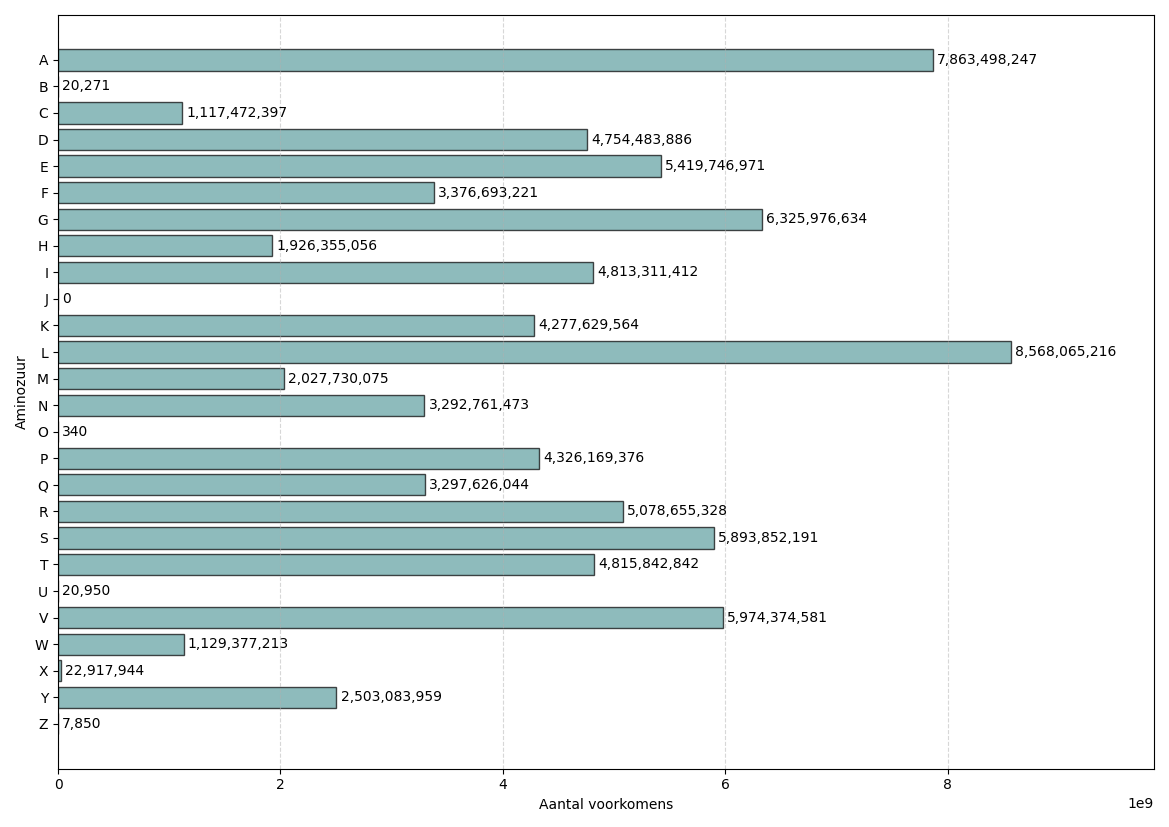
\includegraphics[width=0.6\linewidth]{uniprotKB_aminozuur_voorkomens}
    \caption{Aantal voorkomens per aminozuur voor alle proteïnen in de UniProtKB (2023\_04) databank.}
    \label{fig:uniprot_aminozuur}
\end{figure}

\begin{figure}[h]
    \centering
    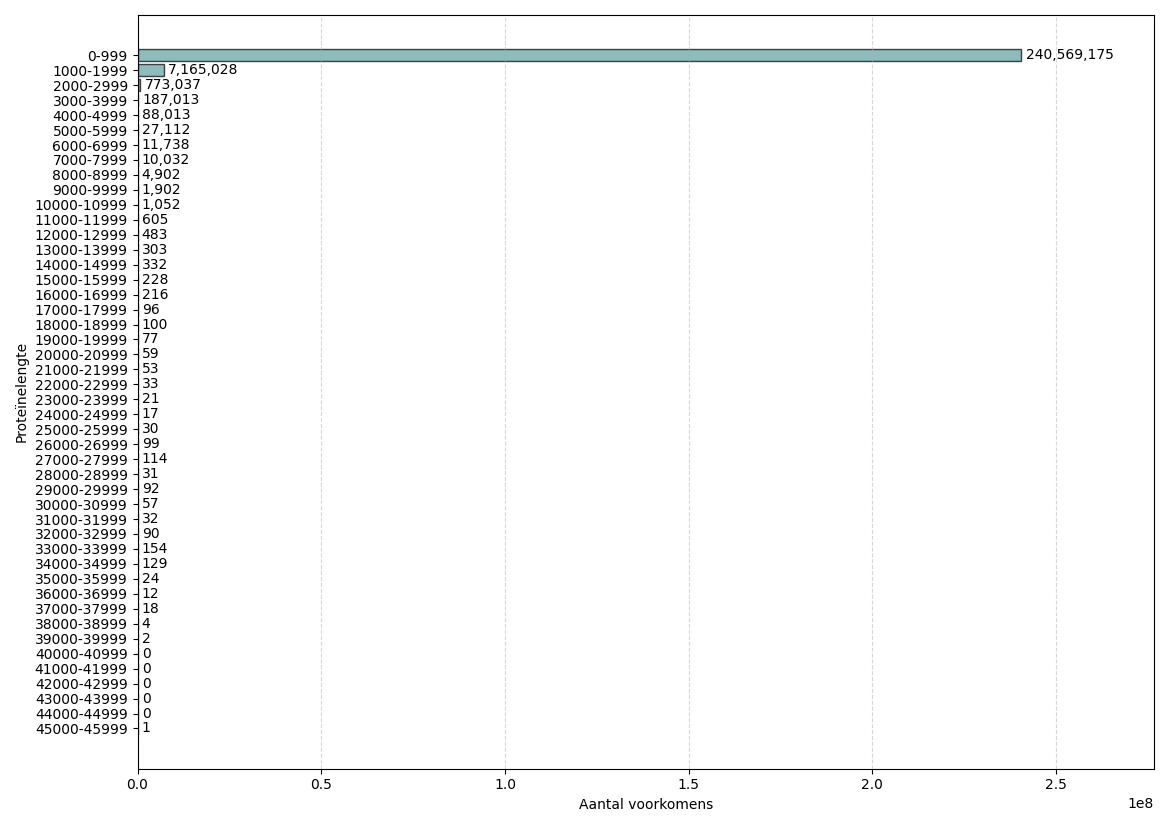
\includegraphics[width=0.95\linewidth]{uniprotKB_length_distribution_large}
    \makebox[0pt][r]{% Similar to \llap
        \raisebox{2.2em}{%
            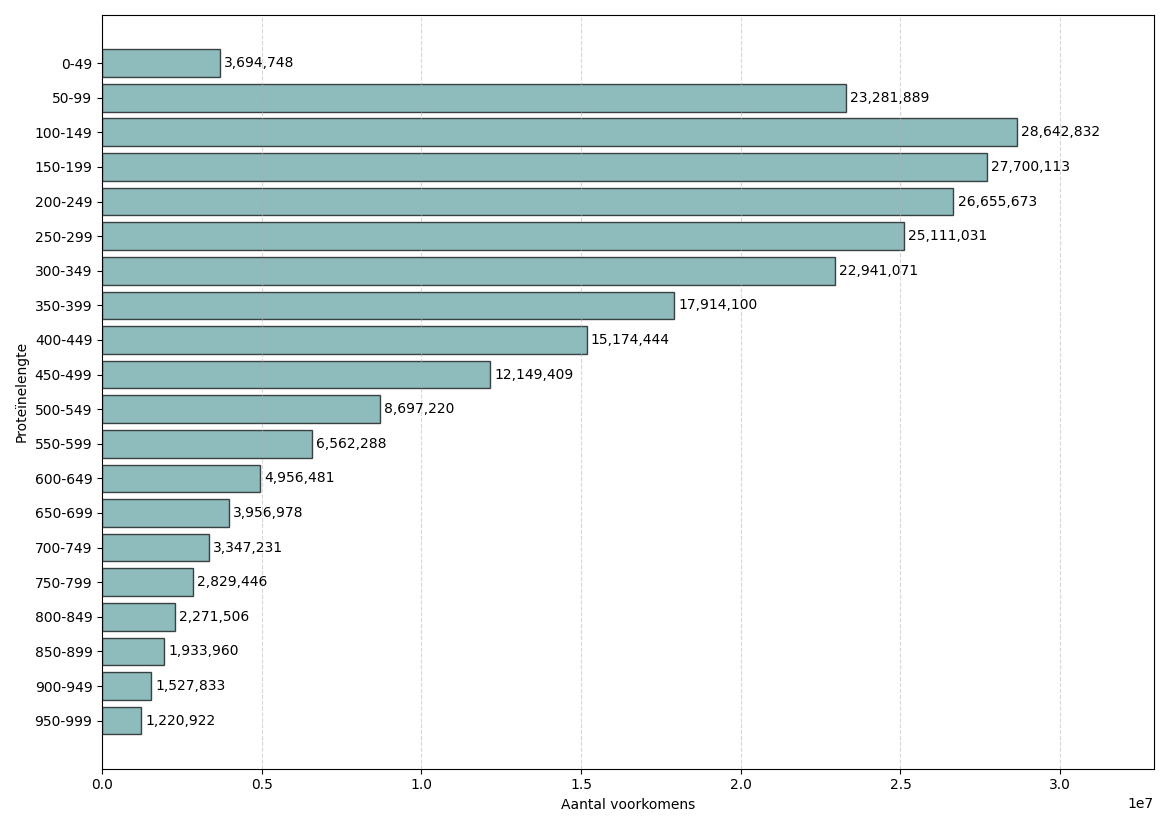
\includegraphics[width=0.65\linewidth]{uniprotKB_length_distribution_small}% Inserted image/inset
        }\hspace*{2em}%
    }%
    \caption{Lengtedistributie van de proteïnen in de UniProtKB (2023\_04) databank. De kleinere grafiek bevat een gedetailleerder overzicht van de distributie in het interval $[0, 1000[$.}\label{fig:uniprot_length}
\end{figure}

\paragraph{Swiss-Prot} De Swiss-Prot databank is één van de twee standaardonderdelen van UniProtKB\@.
Een kort overzicht van alle statistieken is terug te vinden in Tabel~\ref{tab:swissprot_eigenschappen}.
Figuur~\ref{fig:swissprot_aminozuur} en Figuur~\ref{fig:swissprot_length} geven meer inzicht in de distributie van de aminozuren en lengte van de proteïnen.

\begin{table}[h]
    \centering
    \begin{tabular}{l l}
        Metriek                   & Waarde                           \\
        \hline\hline
        Totaal aantal sequenties  & 569\thinspace619                 \\
        Totale lengte             & 205\thinspace954\thinspace074 AA \\
        Minimale proteïnelengte   & 2 AA                             \\
        Maximale proteïnelengte   & 35\thinspace213 AA               \\
        Gemiddelde proteïnelengte & 361.56 AA                        \\
        Mediaan proteïnelengte    & 295 AA                           \\
        \hline
    \end{tabular}
    \caption{Eigenschappen van de Swiss-Prot databank (UniProtKB 2023\_04). De afkorting \textit{AA} staat voor \textit{amino acids}.}
    \label{tab:swissprot_eigenschappen}
\end{table}


\begin{figure}[h]
    \centering
    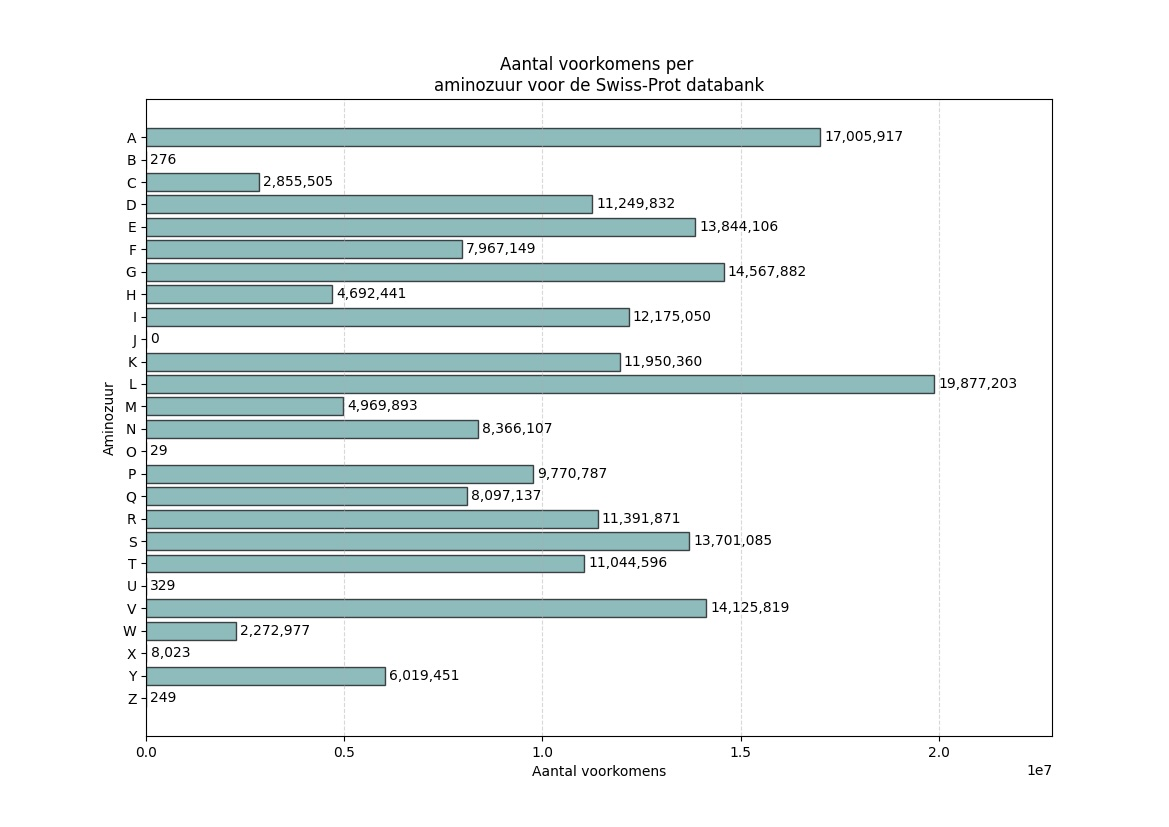
\includegraphics[width=0.6\linewidth]{swissprot_aminozuur_voorkomens}
    \caption{Aantal voorkomens per aminozuur voor alle proteïnen in de Swiss-Prot databank uit UniProtKB 2023\_04. De letters B, J, O, U, X en Z stellen geen aminozuur voor, maar zijn een soort \textit{wildcards} voor meerdere mogelijke aminozuren.}
    \label{fig:swissprot_aminozuur}
\end{figure}

\begin{figure}[h]
    \centering
    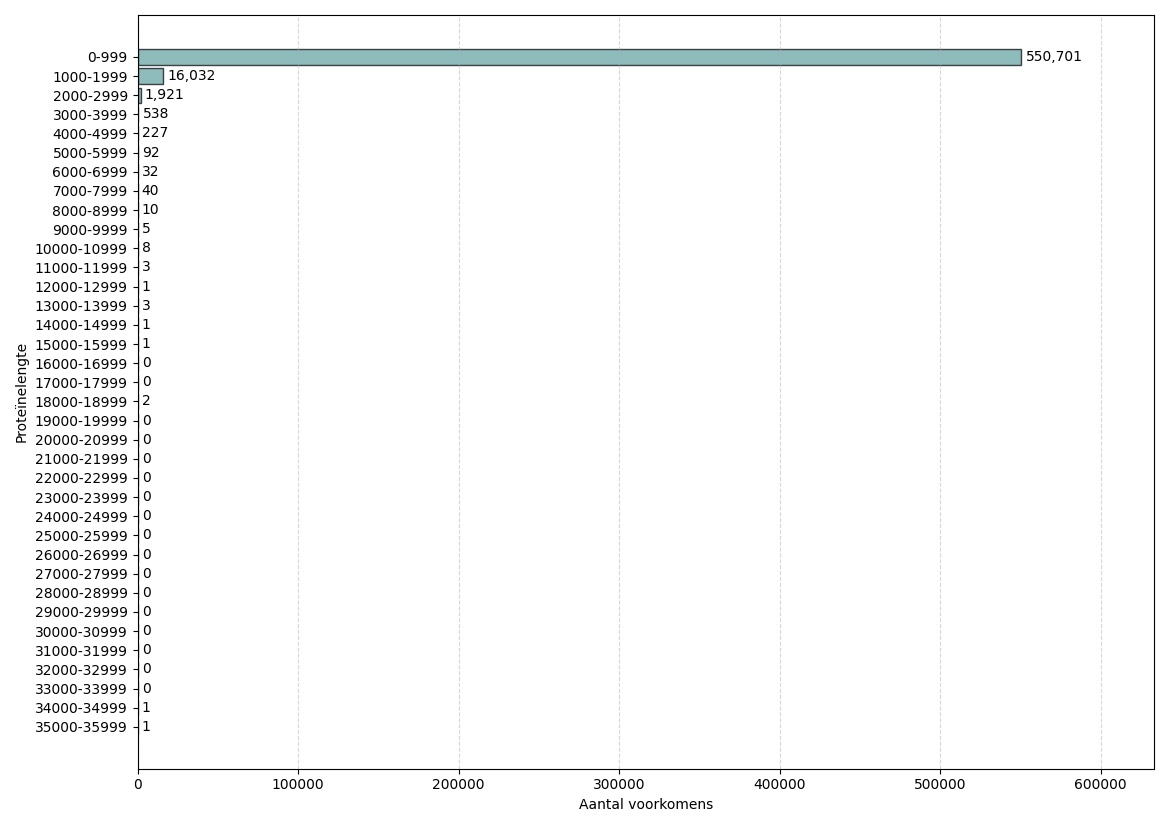
\includegraphics[width=0.95\linewidth]{swissprot_length_distribution_large}
    \makebox[0pt][r]{% Similar to \llap
        \raisebox{2.2em}{%
            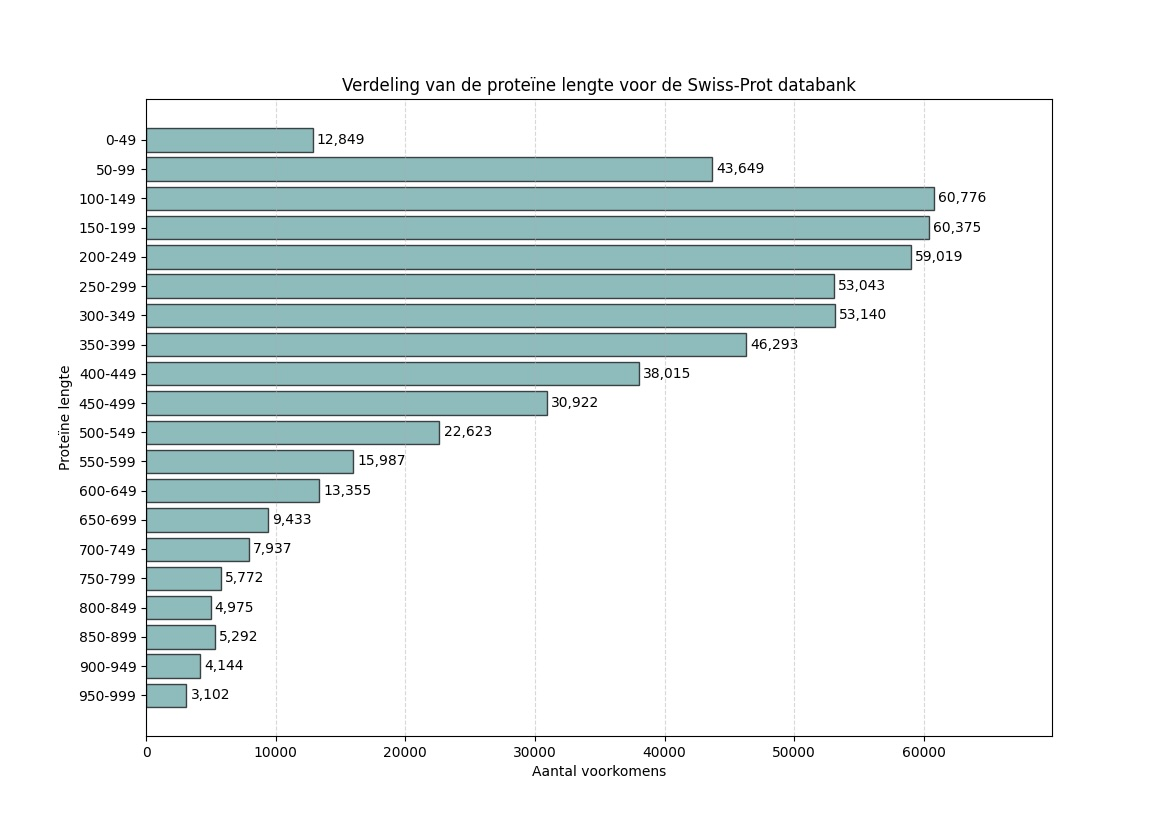
\includegraphics[width=0.65\linewidth]{swissprot_length_distribution_small}% Inserted image/inset
        }\hspace*{2em}%
    }%
    \caption{Lengtedistributie van de proteïnen in de Swiss-Prot databank. De kleinere grafiek bevat een gedetailleerder overzicht van de distributie in het interval $[0, 1000[$.}\label{fig:swissprot_length}
\end{figure}

Doordat het gebruikte invoerbestand reeds verwerkt werd door een deel van de Unipept pipeline, is er een klein verschil tussen het totaal aantal sequenties in Tabel~\ref{tab:swissprot_eigenschappen} en wat eerder aangegeven werd.
Hierbij worden onder andere sequenties met een onbekend taxon id verwijderd (538 in totaal), wat het kleine verschil verklaart.

\paragraph{Human-Prot} De Human-Prot databank is samengesteld aan de hand van drie referentiedatabanken afkomstig uit UniProtKB\@.
Dit zijn de Human Genome~\cite{proteomes_homo_sapiens}, Influenza B~\cite{proteomes_infuenza_b} en Human Papillomavirus~\cite{proteomes_human_papillomavirus} databank.
\\ \\
Deze Human-Prot databank is kleiner dan Swiss-Prot, waardoor het testen tijdens ontwikkeling sneller is.
Tabel~\ref{tab:humanprot_eigenschappen} somt enkele belangrijke metrieken op over deze dataset.
Figuur~\ref{fig:humanprot_aminozuur} en~\ref{fig:humanprot_length} gaan dieper in op de aminozuur- en lengtedistributie van de proteïnen.
\\
\begin{table}[ht]
    \centering
    \begin{tabular}{ l l }
        Metriek                   & Waarde                          \\
        \hline\hline
        Totaal aantal sequenties  & 82\thinspace695                 \\
        Totale lengte             & 30\thinspace293\thinspace046 AA \\
        Minimale proteïnelengte   & 2 AA                            \\
        Maximale proteïnelengte   & 35\thinspace991 AA              \\
        Gemiddelde proteïnelengte & 366.32 AA                       \\
        Mediaan proteïnelengte    & 204 AA                          \\
        \hline
    \end{tabular}
    \caption{Eigenschappen van de Human-Prot databank (UniProtKB 2023\_04). De afkorting \textit{AA} staat voor \textit{amino acids}.}
    \label{tab:humanprot_eigenschappen}
\end{table}

\begin{figure}[ht]
    \centering
    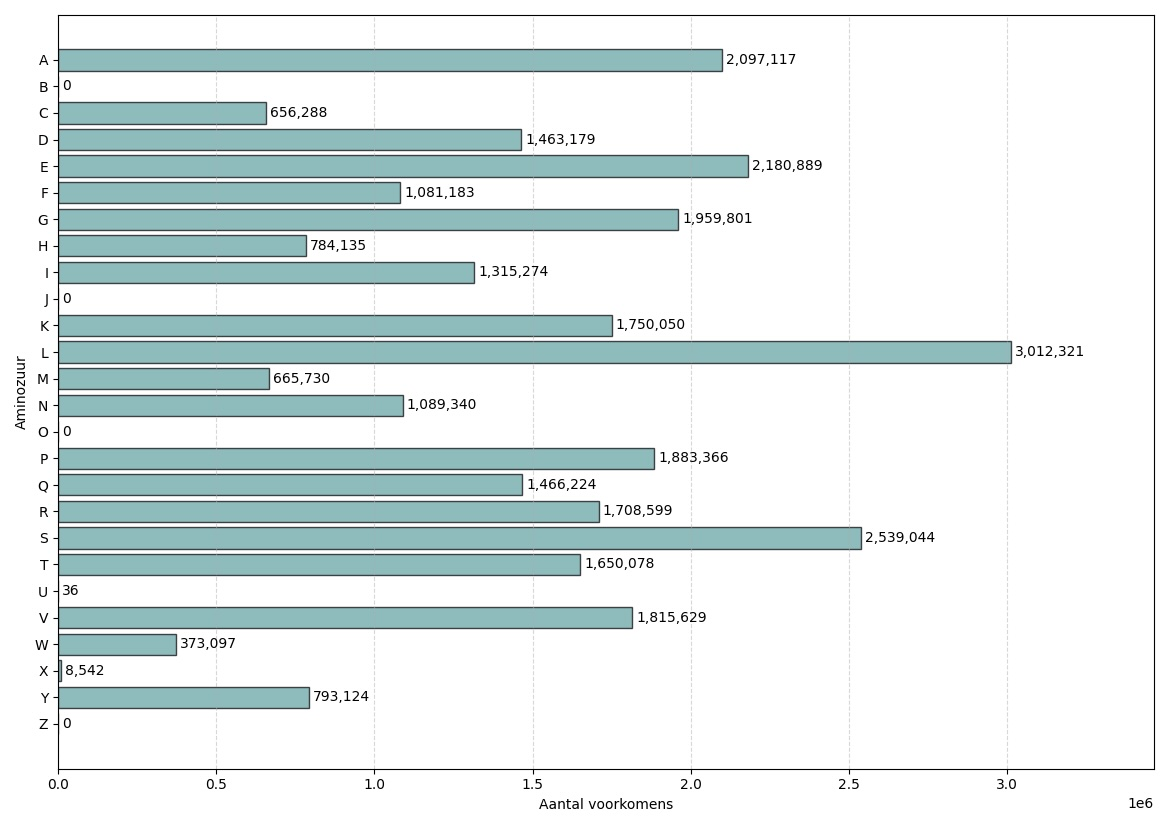
\includegraphics[width=0.7\linewidth]{humanprot_aminozuur_voorkomens}
    \caption{Aantal voorkomens per aminozuur voor alle proteïnen in de Human-Prot databank.}
    \label{fig:humanprot_aminozuur}
\end{figure}

\begin{figure}[ht]
    \centering
    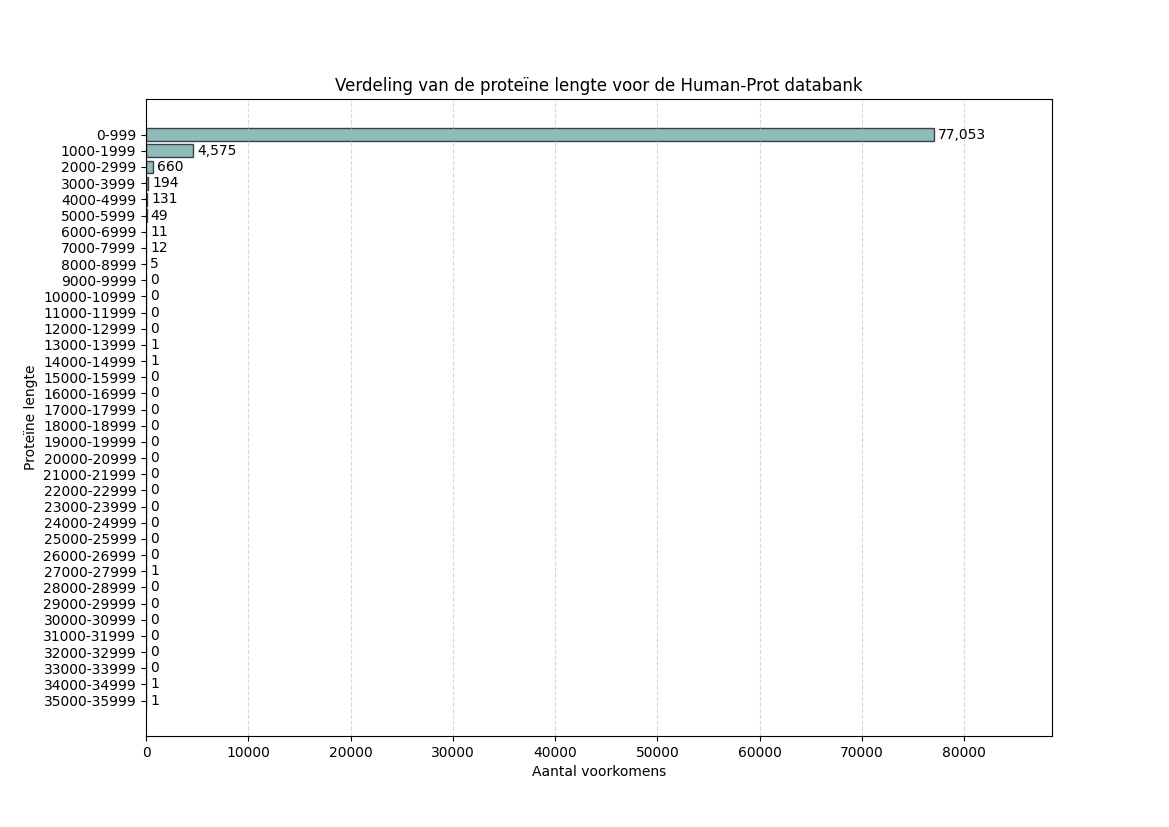
\includegraphics[width=0.95\linewidth]{humanprot_length_distribution_large}
    \makebox[0pt][r]{% Similar to \llap
        \raisebox{2.2em}{%
            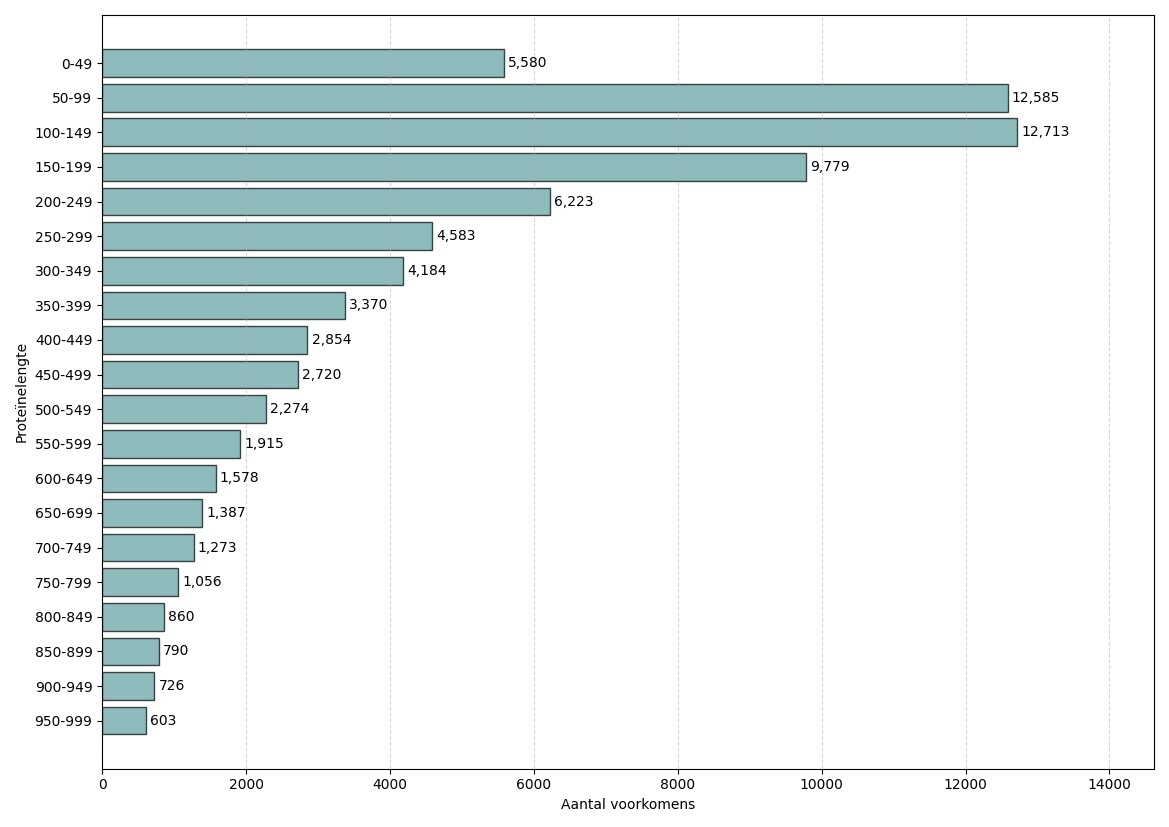
\includegraphics[width=0.65\linewidth]{humanprot_length_distribution_small}% Inserted image/inset
        }\hspace*{2em}%
    }%
    \caption{Lengtedistributie van de proteïnen in de Human-Prot databank. De kleinere grafiek bevat een gedetailleerder overzicht van de distributie in het interval $[0, 1000[$.}\label{fig:humanprot_length}
\end{figure}

We kunnen concluderen dat zo goed als \textbf{alle letters gebruikt} worden (ook al zijn er maar 20 aminozuren).
Dit komt doordat sommige letters eigenlijk een soort wildcard voorstellen.
Zo staat ``X'' voor elk mogelijk aminozuur, ``Z'' voor ``Q'' of ``E'',\ldots~\cite{amino_acid_codes}.
\\ \\
Verder valt ook te zien dat de verdeling van de proteïnelengtes in de UniProtKB, Swiss-Prot en Human-Prot datasets vergelijkbaar zijn.
Met andere woorden: \textbf{Swiss-Prot en Human-Prot zijn een representatieve kleinere voorstelling van UniProtKB\@}.
Dit laat ons toe om gebruik te maken van de Swiss-Prot en Human-Prot proteïnedatabanken en later de resultaten te veralgemenen en op te schalen naar UniProtKB\@.

\subsection{Peptidebestanden}\label{subsec:peptide-zoek-bestanden}
De zoekperformantie van onze indexstructuur is een erg belangrijk aspect.
Om dit te meten, hebben we bij elke proteïnedatabank een lijst van peptiden die we proberen te zoeken.
Zowel voor de Swiss-Prot als Human-Prot databank zijn enkele datasets opgesteld.

\subsubsection{Swiss-Prot}
Voor deze proteïnedatabank hebben we enkele peptidebestanden voorzien.
Twee bestanden die gesampled zijn en een reeks aan real-life stalen.
De twee artificiële bestanden zijn zo gekozen dat de ene enkel tryptische peptiden bevat, terwijl de andere ook peptiden bevat met \textit{missed cleavages}.
De eerste kan dus op dit moment al efficiënt door Unipept verwerkt worden, terwijl dit voor de tweede onmogelijk is.

\paragraph{Artificiële stalen}
Tabel~\ref{tab:artifiele_bestanden_statistieken} bevat in kolom twee en drie een kort overzicht met statistieken voor deze gesamplede bestanden.

\begin{table}[H]
    \centering
    \begin{tabular}{l l l l}
        Metriek                    & Swiss-Prot-TRYP                & Swiss-Prot-MC                  & Human-Prot                                  \\
        \hline\hline
        Totaal aantal sequenties   & 100\thinspace000               & 100\thinspace000               & 250\thinspace000                            \\
        Totale lengte              & 1\thinspace605\thinspace909 AA & 2\thinspace544\thinspace356 AA & 2\thinspace458\thinspace834\thinspace046 AA \\
        Minimale peptidelengte     & 5 AA                           & 5 AA                           & 1 AA                                        \\
        Maximale peptidelengte     & 50 AA                          & 93 AA                          & 12 AA                                       \\
        Gemiddelde peptidelengte   & 16.06 AA                       & 25.44 AA                       & 9.84 AA                                     \\
        Mediaan peptidelengte      & 13 AA                          & 23 AA                          & 10 AA                                       \\
        Aantal vindbare peptiden   & 67\thinspace375                & 62\thinspace581                & 250\thinspace000                            \\
        Aantal tryptische peptiden & 100\thinspace000               & 4107                           & 102\thinspace659                            \\
        \hline
    \end{tabular}
    \caption{Eigenschappen van de verschillende peptidebestanden. \textit{Swiss-Prot-TRYP} bevat de statistieken voor het Swiss-Prot peptidebestand met enkel tryptische peptiden. Hierbij komen er dus geen \textit{missed cleavages} voor. \textit{Swiss-Prot-MC} bevat net wel \textit{missed cleavages}. De laatste kolom bevat de statistieken voor het peptidebestand dat hoort bij de Human-Prot proteïnedatabank. De afkorting \textit{AA} staat voor \textit{amino acids}.}
    \label{tab:artifiele_bestanden_statistieken}
\end{table}

\paragraph{Experimentele stalen}
Om de performantie beter te beoordelen, gebruiken we ook enkele stalen uit experimenten met een kleine micro-organisme gemeenschap, namelijk SIHUMIx\footnote{Simplified human intestinal microbiota}~\cite{SIHUMI_first_introduction, SIHUMI_frequently_used}.
Aangezien deze stalen uit een experiment ontstaan zijn, bevatten deze \textit{missed cleavages} die natuurlijk ontstaan zijn.
De peptiden zijn dus effectief ontstaan uit een staal proteïnen waarop trypsine toegepast is.
Tabel~\ref{tab:sihumi_zoekbestanden} bevat de belangrijkste statistieken voor elk peptidebestand.
Deze peptidebestanden worden in combinatie met de Swiss-Prot proteïnedatabank gebruikt tijdens het testen.

\begin{table}[H]
    \begin{minipage}{\linewidth}
        \centering
        \resizebox{\textwidth}{!}{ % use resizebox to textwidth since this needs to be scaled down in size a bit because otherwise it does not fit on the width of the screen
            \begin{tabular}{ l l l l l l l }
                Metriek                    & SIHUMI 03           & SIHUMI 05           & SIHUMI 05           & SIHUMI 08           & SIHUMI 11           & SIHUMI 14           \\
                \hline\hline
                Totaal aantal sequenties   & 25\thinspace000     & 25\thinspace000     & 24\thinspace424     & 25\thinspace000     & 24\thinspace998     & 25\thinspace000     \\
                Totale lengte              & 420\thinspace544 AA & 420\thinspace423 AA & 373\thinspace633 AA & 316\thinspace114 AA & 366\thinspace894 AA & 430\thinspace674 AA \\
                Minimale peptidelengte     & 6 AA                & 6 AA                & 6 AA                & 6 AA                & 6 AA                & 6 AA                \\
                Maximale peptidelengte     & 50 AA               & 50 AA               & 47 AA               & 43 AA               & 50 AA               & 50 AA               \\
                Gemiddelde peptidelengte   & 16.82 AA            & 16.82 AA            & 15.30 AA            & 12.64 AA            & 14.68 AA            & 17.23 AA            \\
                Mediaan peptidelengte      & 15 AA               & 16 AA               & 14 AA               & 12 AA               & 14 AA               & 16 AA               \\
                Aantal vindbare peptiden   & 2570                & 2698                & 3652                & 4135                & 3792                & 2761                \\
                Aantal tryptische peptiden & 17\thinspace263     & 162                 & 152                 & 207                 & 153                 & 242                 \\
                \hline
            \end{tabular}}
        \caption{Eigenschappen van de SIHUMIx peptidebestanden. Elke kolom stelt een staal voor met als bestandsnaam \texttt{S<XX>.txt}. Deze stalen kunnen teruggevonden worden in onze GitHub repository\protect\footnote{\url{https://github.com/BramDevlaminck/Thesis\_benchmarkdata}} onder de \texttt{SIHUMI}-folder. De afkorting \textit{AA} staat voor \textit{amino acids}.} % protect is needed to make footnote possible in a caption. This is combined with a minipage to place the footnote directly under the table
        \label{tab:sihumi_zoekbestanden}
    \end{minipage}
\end{table}

\subsubsection{Human-Prot}
Voor deze databank hebben we één peptidebestand waarin we HLA-peptiden simuleren.
Dit zijn \textbf{korte, niet-tryptische peptiden} waarin men typisch geïnteresseerd is in het immunopeptidomics onderzoeksveld~\cite{immunopeptidomics}.
Dit betekent dat Unipept op dit moment niet gebruikt kan worden om dit soort stalen te analyseren.
Elke peptide in dit peptidebestand is een sample van een proteïne uit de Human-Prot databank.
Hierdoor zijn alle peptiden die we zoeken effectief vindbaar in de dataset.
Een kort overzicht van de eigenschappen is terug te vinden in de laatste kolom van Tabel~\ref{tab:artifiele_bestanden_statistieken}.
\\ \\
Appendix~\ref{ch:appendix-statistieken-peptidebestanden} bevat aanvullende grafieken over bovenstaande peptidebestanden.
Deze tonen voor elk bestand de distributie van de aminozuren en peptidelengte.
% TODO: hier ergens vermelden als apart onderdeeltje hoeveel geheugen nodig is op dit moment voor swissprot in unipept om index op te bouwen, hoe lang dit duurt, en hoe lang het zoeken tot match duurt voor swissprot met en zonder missed cleavage


\section{Benchmark hardware}\label{sec:benchmark-hardware}
Alle benchmarks werden uitgevoerd op een virtuele machine van team Unipept tenzij anders vermeld.
Tabel~\ref{tab:Matt_hardware} bevat een overzicht van de hardware van de fysieke machine en hoeveel toegekend is aan de VM\@.
Alle informatie omtrent Unipept infrastructuur kan teruggevonden worden op de Unipept GitHub wiki~\cite{unipept_infrastructure}.
\\ \\
Een deel van de kleinere testen werd ook lokaal uitgevoerd op een laptop.
Dit zal elke keer expliciet vermeld worden indien dit het geval was.
De gebruikte laptop is een M1 Pro MacBook Pro (14 inch) uit 2021.
Tabel~\ref{tab:macbook_hardware} bevat de exacte specificaties van deze laptop.
\\ \\
Naast een VM en eigen laptop hebben we ook toegang tot enkele andere machines indien hier nood toe zou zijn.
Een eerste mogelijke optie is via een andere, krachtigere server van Unipept.
Het mogelijk om applicaties die op dit moment op verschillend servers draaien, tijdelijk te herverdelen zodat er een machine met 768 GiB ram ter beschikking komt.
Een andere optie is de HPC van UGent\footnote{\url{https://docs.hpc.ugent.be/}}.
Hierop zijn nodes\footnote{Elke node bestaat is een fysieke server. Deze nodes vormen samen een cluster op de HPC.} beschikbaar tot 940 GiB RAM\@.
Tot slot heeft de CompOmics\footnote{Computational Omics} onderzoeksgroep aan UGent ook enkele machines staan die tot 2 TiB aan geheugen hebben.
Deze onderzoeksgroep werkt aan softwaretoepassingen voor het verwerken van proteomica-data, waar het onderzoeksgebied van de metaproteomica onder valt.

\begin{table}[ht]
    \centering
    \begin{tabular}{p{0.20\linewidth}p{0.45\linewidth}p{0.25\linewidth}}
        Onderdeel         & Fysieke server                                                                      & Virtuele Machine     \\
        \hline\hline
        CPU               & 2\times Intel Xeon 4410Y (12 cores / 24 threads, 2 - 3.9 GhZ, 30 MiB cache)         & 12 threads           \\
        RAM               & 768 GiB                                                                             & 128 GiB              \\
        Opslag            & 6\times 16 TiB HDD (3.5 inch, 7.2K RPM SATA), 4\times 3.84 TiB SSD (2.5 inch, SATA) & 1 TiB SSD, 4 TiB HDD \\
        Besturingssysteem & Debian 12 (met Proxmox)                                                             & Ubuntu 22.04 LTS     \\
        \hline
    \end{tabular}
    \caption{Hardwarespecificaties van de fysieke server en virtuele machine die gebruikt worden tijdens het testen. Deze virtuele machine draait samen met enkele andere VMs op de server.}
    \label{tab:Matt_hardware}
\end{table}

\begin{table}[ht]
    \centering
    \begin{tabular}{p{0.20\linewidth}p{0.54\linewidth}}
        Onderdeel         & hardware                                               \\
        \hline\hline
        Model             & MacBook Pro (14 inch, 2021)                            \\
        CPU               & 8-core M1 Pro, 6 performance cores, 2 efficiency cores \\
        RAM               & 16 GB (LPDDR5)                                         \\
        Opslag            & 512 GB SSD                                             \\
        Besturingssysteem & MacOS (14) Sonoma                                      \\
        \hline
    \end{tabular}
    \caption{Hardwarespecificaties van de gebruikte laptop voor kleinere testen.}
    \label{tab:macbook_hardware}
\end{table}

\section{Mogelijke oplossingen}\label{sec:mogelijke-oplossingen}
De essentie van onze probleemstelling is het snel vinden van een grote hoeveelheid korte strings in één erg lange string.
Dit is een vorm van stringmatching.
Hiervoor bestaan twee verschillende strategieën (die ook gecombineerd kunnen worden).
\begin{enumerate}
    \item \textbf{Verwerk de korte zoekstring op voorhand} (van lengte $n$) zoals in het algoritme van Knuth-Morris-Pratt~\cite{knuth-morris-pratt}, Boyer-Moore-Horspool~\cite{boyer-moore-horspool} en het shift-AND-algoritme~\cite{shift-and}.
    \item \textbf{Verwerk de lange tekst op voorhand} (van lengte $m$) zoals bij suffixbomen~\cite{mcCreight_first_suffixtree}, suffix arrays~\cite{suffix_array_first_mention} en (bidirectionele) FM-indices~\cite{fm_index, bi-directional_fm_index}.
\end{enumerate}

Voor beide strategieën bestaan er algoritmen die in lineaire tijd ten opzichte van de stringlengte een indexstructuur bouwen, en deze kunnen doorzoeken.
Er is echter een belangrijk verschil.
\\ \\
Bij de strategie waar we de korte zoekstring op voorhand verwerken kan het opbouwen in $O(n)$ tijd en geheugen, en het zoeken in $O(m)$ tijd (met $n$ de lengte van de zoekstring, en $m$ de lengte van de tekst).
Hierbij is het \textbf{zoeken} dus \textbf{lineair in de tijd ten opzichte van de lengte van de totale tekst}.
Dit is nadelig wanneer er veel korte strings zijn, waarvoor elke keer extra werk moet gebeuren.
Daarna moeten we bovendien nog voor elke korte string de zoekoperatie uitvoeren, waarvoor de uitvoeringstijd lineair is in de lengte van de volledige tekst.
\\ \\
Indien we de lange tekst indexeren, kan het opbouwen in $O(m)$ tijd en het zoeken in $O(n)$ tijd en geheugen (opnieuw met $n$ de lengte van de zoekstring, en $m$ de lengte van de tekst).
Hierbij is het mogelijk om één keer de indexstructuur te bouwen voor de lange tekst, waarna elke korte string \textbf{in lineaire tijd ten opzichte van zijn eigen lengte gezocht} kan worden.
Het nadeel is echter dat het opbouwen van de indexstructuur voor een grote tekst traag kan worden, en bovendien veel geheugen kan innemen.
\\ \\
We hebben een grote databank met erg veel proteïnen (een lange tekst) waarin we erg veel peptiden (korte strings) zoeken, wat overeenkomt met de tweede aanpak.
Daarom verkennen we in deze masterproef die aanpak.
In de eerste instantie willen we \textbf{exacte matches} kunnen zoeken, maar later willen we ook \textbf{inexacte} \textit{matching} uitvoeren.
\\ \\
Aangezien de indexstructuur slechts eenmalig voor een bepaalde proteïnedatabank opgebouwd moet worden, ligt de \textbf{primaire restrictie bij het geheugengebruik} tijdens het opbouwen.
Het blijft echter steeds belangrijk dat de indexstructuur in een redelijke tijd opgebouwd kan worden en performant genoeg is om snel een groot aantal peptiden te zoeken.
De richttijd die we ons vooropstellen om de indexstructuur op te bouwen voor UniProtKB is maximaal één à twee dagen.
Dit is een acceptabele tijdsduur aangezien de indexstructuur slechts om de acht weken opnieuw opgebouwd moet worden, overeenkomstig met de frequentie waarbij een nieuwe versie van de UniProtKB databank uitgebracht wordt.
In de volgende hoofdstukken verkennen we verschillende indexstructuren om een proteïnedatabank te indexeren.